%%%%%%%%%%%%%%%%%%%%%%%%%%%%%%%%%%%%%%%%%%%%%%%%%%%%%%%%%%%%%%%%%%%%%%
% Template for a UBC-compliant dissertation
% At the minimum, you will need to change the information found
% after the "Document meta-data"
%
%!TEX TS-program = pdflatex
%!TEX encoding = UTF-8 Unicode

%% The ubcdiss class provides several options:
%%   gpscopy (aka fogscopy)
%%       set parameters to exactly how GPS specifies
%%         * single-sided
%%         * page-numbering starts from title page
%%         * the lists of figures and tables have each entry prefixed
%%           with 'Figure' or 'Table'
%%       This can be tested by `\ifgpscopy ... \else ... \fi'
%%   10pt, 11pt, 12pt
%%       set default font size
%%   oneside, twoside
%%       whether to format for single-sided or double-sided printing
%%   balanced
%%       when double-sided, ensure page content is centred
%%       rather than slightly offset (the default)
%%   singlespacing, onehalfspacing, doublespacing
%%       set default inter-line text spacing; the ubcdiss class
%%       provides \textspacing to revert to this configured spacing
%%   draft
%%       disable more intensive processing, such as including
%%       graphics, etc.
%%

% For submission to GPS
\documentclass[gpscopy,onehalfspacing,11pt]{ubcdiss}
% For your own copies (looks nicer)
% \documentclass[balanced,twoside,11pt]{ubcdiss}

%%%%%%%%%%%%%%%%%%%%%%%%%%%%%%%%%%%%%%%%%%%%%%%%%%%%%%%%%%%%%%%%%%%%%%
%%%%%%%%%%%%%%%%%%%%%%%%%%%%%%%%%%%%%%%%%%%%%%%%%%%%%%%%%%%%%%%%%%%%%%
%%
%% FONTS:
%% 
%% The defaults below configures Times Roman for the serif font,
%% Helvetica for the sans serif font, and Courier for the
%% typewriter-style font.  Configuring fonts can be time
%% consuming; we recommend skipping to END FONTS!
%% 
%% If you're feeling brave, have lots of time, and wish to use one
%% your platform's native fonts, see the commented out bits below for
%% XeTeX/XeLaTeX.  This is not for the faint at heart. 
%% (And shouldn't you be writing? :-)
%%

%% NFSS font specification (New Font Selection Scheme)
\usepackage{times,mathptmx,courier}
\usepackage[scaled=.92]{helvet}

%% Math or theory people may want to include the handy AMS macros
\usepackage{amssymb} % for $\mathbb{R}$, Real R
%\usepackage{amsmath}
%\usepackage{amsfonts}

%% The pifont package provides access to the elements in the dingbat font.   
%% Use \ding{##} for a particular dingbat (see p7 of psnfss2e.pdf)
%%   Useful:
%%     51,52 different forms of a checkmark
%%     54,55,56 different forms of a cross (saltyre)
%%     172-181 are 1-10 in open circle (serif)
%%     182-191 are 1-10 black circle (serif)
%%     192-201 are 1-10 in open circle (sans serif)
%%     202-211 are 1-10 in black circle (sans serif)
%% \begin{dinglist}{##}\item... or dingautolist (which auto-increments)
%% to create a bullet list with the provided character.
\usepackage{pifont}

%%%%%%%%%%%%%%%%%%%%%%%%%%%%%%%%%%%%%%%%%%%%%%%%%%%%%%%%%%%%%%%%%%%%%%
%% Configure fonts for XeTeX / XeLaTeX using the fontspec package.
%% Be sure to check out the fontspec documentation.
%\usepackage{fontspec,xltxtra,xunicode}	% required
%\defaultfontfeatures{Mapping=tex-text}	% recommended
%% Minion Pro and Myriad Pro are shipped with some versions of
%% Adobe Reader.  Adobe representatives have commented that these
%% fonts can be used outside of Adobe Reader.
%\setromanfont[Numbers=OldStyle]{Minion Pro}
%\setsansfont[Numbers=OldStyle,Scale=MatchLowercase]{Myriad Pro}
%\setmonofont[Scale=MatchLowercase]{Andale Mono}

%% Other alternatives:
%\setromanfont[Mapping=tex-text]{Adobe Caslon}
%\setsansfont[Scale=MatchLowercase]{Gill Sans}
%\setsansfont[Scale=MatchLowercase,Mapping=tex-text]{Futura}
%\setmonofont[Scale=MatchLowercase]{Andale Mono}
%\newfontfamily{\SYM}[Scale=0.9]{Zapf Dingbats}
%% END FONTS
%%%%%%%%%%%%%%%%%%%%%%%%%%%%%%%%%%%%%%%%%%%%%%%%%%%%%%%%%%%%%%%%%%%%%%
%%%%%%%%%%%%%%%%%%%%%%%%%%%%%%%%%%%%%%%%%%%%%%%%%%%%%%%%%%%%%%%%%%%%%%



%%%%%%%%%%%%%%%%%%%%%%%%%%%%%%%%%%%%%%%%%%%%%%%%%%%%%%%%%%%%%%%%%%%%%%
%%%%%%%%%%%%%%%%%%%%%%%%%%%%%%%%%%%%%%%%%%%%%%%%%%%%%%%%%%%%%%%%%%%%%%
%%
%% Recommended packages
%%
\usepackage{checkend}	% better error messages on left-open environments
\usepackage{graphicx}	% for incorporating external images

%% booktabs: provides some special commands for typesetting tables as used
%% in excellent journals.  Ignore the examples in the Lamport book!
\usepackage{booktabs}

%% listings: useful support for including source code listings, with
%% optional special keyword formatting.  The \lstset{} causes
%% the text to be typeset in a smaller sans serif font, with
%% proportional spacing.
\usepackage{listings}
\lstset{basicstyle=\sffamily\scriptsize,showstringspaces=false,fontadjust}

%% The acronym package provides support for defining acronyms, providing
%% their expansion when first used, and building glossaries.  See the
%% example in glossary.tex and the example usage throughout the example
%% document.
%% NOTE: to use \MakeTextLowercase in the \acsfont command below,
%%   we *must* use the `nohyperlinks' option -- it causes errors with
%%   hyperref otherwise.  See Section 5.2 in the ``LaTeX 2e for Class
%%   and Package Writers Guide'' (clsguide.pdf) for details.
\usepackage[printonlyused,nohyperlinks]{acronym}
%% The ubcdiss.cls loads the `textcase' package which provides commands
%% for upper-casing and lower-casing text.  The following causes
%% the acronym package to typeset acronyms in small-caps
%% as recommended by Bringhurst.
\renewcommand{\acsfont}[1]{{\scshape \MakeTextLowercase{#1}}}

%% color: add support for expressing colour models.  Grey can be used
%% to great effect to emphasize other parts of a graphic or text.
%% For an excellent set of examples, see Tufte's "Visual Display of
%% Quantitative Information" or "Envisioning Information".
\usepackage{color}
\definecolor{greytext}{gray}{0.5}

%% comment: provides a new {comment} environment: all text inside the
%% environment is ignored.
%%   \begin{comment} ignored text ... \end{comment}
\usepackage{comment}

%% The natbib package provides more sophisticated citing commands
%% such as \citeauthor{} to provide the author names of a work,
%% \citet{} to produce an author-and-reference citation,
%% \citep{} to produce a parenthetical citation.
%% We use \citeeg{} to provide examples
\usepackage[numbers,sort&compress]{natbib}
\newcommand{\citeeg}[1]{\citep[e.g.,][]{#1}}

%% The titlesec package provides commands to vary how chapter and
%% section titles are typeset.  The following uses more compact
%% spacings above and below the title.  The titleformat that follow
%% ensure chapter/section titles are set in singlespace.
\usepackage[compact]{titlesec}
\titleformat*{\section}{\singlespacing\raggedright\bfseries\Large}
\titleformat*{\subsection}{\singlespacing\raggedright\bfseries\large}
\titleformat*{\subsubsection}{\singlespacing\raggedright\bfseries}
\titleformat*{\paragraph}{\singlespacing\raggedright\itshape}

%% The caption package provides support for varying how table and
%% figure captions are typeset.
\usepackage[format=hang,indention=-1cm,labelfont={bf},margin=1em]{caption}

%% url: for typesetting URLs and smart(er) hyphenation.
%% \url{http://...} 
\usepackage{url}
\urlstyle{sf}	% typeset urls in sans-serif


%%%%%%%%%%%%%%%%%%%%%%%%%%%%%%%%%%%%%%%%%%%%%%%%%%%%%%%%%%%%%%%%%%%%%%
%%%%%%%%%%%%%%%%%%%%%%%%%%%%%%%%%%%%%%%%%%%%%%%%%%%%%%%%%%%%%%%%%%%%%%
%%
%% Possibly useful packages: you may need to explicitly install
%% these from CTAN if they aren't part of your distribution;
%% teTeX seems to ship with a smaller base than MikTeX and MacTeX.
%%
%\usepackage{pdfpages}	% insert pages from other PDF files
%\usepackage{longtable}	% provide tables spanning multiple pages
%\usepackage{chngpage}	% support changing the page widths on demand
%\usepackage{tabularx}	% an enhanced tabular environment

%% enumitem: support pausing and resuming enumerate environments.
%\usepackage{enumitem}

%% rotating: provides two environments, sidewaystable and sidewaysfigure,
%% for typesetting tables and figures in landscape mode.  
%\usepackage{rotating}

%% subfig: provides for including subfigures within a figure,
%% and includes being able to separately reference the subfigures.
%\usepackage{subfig}

%% ragged2e: provides several new new commands \Centering, \RaggedLeft,
%% \RaggedRight and \justifying and new environments Center, FlushLeft,
%% FlushRight and justify, which set ragged text and are easily
%% configurable to allow hyphenation.
%\usepackage{ragged2e}

%% The ulem package provides a \sout{} for striking out text and
%% \xout for crossing out text.  The normalem and normalbf are
%% necessary as the package messes with the emphasis and bold fonts
%% otherwise.
%\usepackage[normalem,normalbf]{ulem}    % for \sout

%%%%%%%%%%%%%%%%%%%%%%%%%%%%%%%%%%%%%%%%%%%%%%%%%%%%%%%%%%%%%%%%%%%%%%
%% HYPERREF:
%% The hyperref package provides for embedding hyperlinks into your
%% document.  By default the table of contents, references, citations,
%% and footnotes are hyperlinked.
%%
%% Hyperref provides a very handy command for doing cross-references:
%% \autoref{}.  This is similar to \ref{} and \pageref{} except that
%% it automagically puts in the *type* of reference.  For example,
%% referencing a figure's label will put the text `Figure 3.4'.
%% And the text will be hyperlinked to the appropriate place in the
%% document.
%%
%% Generally hyperref should appear after most other packages

%% The following puts hyperlinks in very faint grey boxes.
%% The `pagebackref' causes the references in the bibliography to have
%% back-references to the citing page; `backref' puts the citing section
%% number.  See further below for other examples of using hyperref.
%% 2009/12/09: now use `linktocpage' (Jacek Kisynski): GPS now prefers
%%   that the ToC, LoF, LoT place the hyperlink on the page number,
%%   rather than the entry text.
\usepackage[bookmarks,bookmarksnumbered,%
    allbordercolors={0.8 0.8 0.8},%
    pagebackref,linktocpage%
    ]{hyperref}
%% The following change how the the back-references text is typeset in a
%% bibliography when `backref' or `pagebackref' are used
\renewcommand\backrefpagesname{\(\rightarrow\) pages}
\renewcommand\backref{\textcolor{greytext} \backrefpagesname\ }

%% The following uses most defaults, which causes hyperlinks to be
%% surrounded by colourful boxes; the colours are only visible in
%% PDFs and don't show up when printed:
%\usepackage[bookmarks,bookmarksnumbered]{hyperref}

%% The following disables the colourful boxes around hyperlinks.
%\usepackage[bookmarks,bookmarksnumbered,pdfborder={0 0 0}]{hyperref}

%% The following disables all hyperlinking, but still enabled use of
%% \autoref{}
%\usepackage[draft]{hyperref}

%% The following commands causes chapter and section references to
%% uppercase the part name.
\renewcommand{\chapterautorefname}{Chapter}
\renewcommand{\sectionautorefname}{Section}
\renewcommand{\subsectionautorefname}{Section}
\renewcommand{\subsubsectionautorefname}{Section}

%% If you have long page numbers (e.g., roman numbers in the 
%% preliminary pages for page 28 = xxviii), you might need to
%% uncomment the following and tweak the \@pnumwidth length
%% (default: 1.55em).  See the tocloft documentation at
%% http://www.ctan.org/tex-archive/macros/latex/contrib/tocloft/
% \makeatletter
% \renewcommand{\@pnumwidth}{3em}
% \makeatother

%%%%%%%%%%%%%%%%%%%%%%%%%%%%%%%%%%%%%%%%%%%%%%%%%%%%%%%%%%%%%%%%%%%%%%
%%%%%%%%%%%%%%%%%%%%%%%%%%%%%%%%%%%%%%%%%%%%%%%%%%%%%%%%%%%%%%%%%%%%%%
%%
%% Some special settings that controls how text is typeset
%%
% \raggedbottom		% pages don't have to line up nicely on the last line
% \sloppy		% be a bit more relaxed in inter-word spacing
% \clubpenalty=10000	% try harder to avoid orphans
% \widowpenalty=10000	% try harder to avoid widows
% \tolerance=1000


%%%%%%%%%%%%%%%%%%%%%%%%%%%%%%%%%%%%%%%%%%%%%%%%%%%%%%%%%%%%%%%%%%%%%%
%%%%%%%%%%%%%%%%%%%%%%%%%%%%%%%%%%%%%%%%%%%%%%%%%%%%%%%%%%%%%%%%%%%%%%
%%
%% Document meta-data: be sure to also change the \hypersetup information
%%

\title{Master's Thesis Draft}
%\subtitle{If you want a subtitle}

\author{Victor Gan}
\previousdegree{BSc, University of Waterloo, 2013}

% What is this dissertation for?
\degreetitle{Master of Science}

\institution{The University of British Columbia}
\campus{Vancouver}

\faculty{The Faculty of Science}
\department{Computer Science}
\submissionmonth{April}
\submissionyear{2015}

%% hyperref package provides support for embedding meta-data in .PDF
%% files
\hypersetup{
  pdftitle={Change this title!  (DRAFT: \today)},
  pdfauthor={Victor Gan},
  pdfkeywords={Your keywords here}
}

%%%%%%%%%%%%%%%%%%%%%%%%%%%%%%%%%%%%%%%%%%%%%%%%%%%%%%%%%%%%%%%%%%%%%%
%%%%%%%%%%%%%%%%%%%%%%%%%%%%%%%%%%%%%%%%%%%%%%%%%%%%%%%%%%%%%%%%%%%%%%
%% 
%% The document content
%%



%%%%%%%%%%%%%%%%%%%%%%%%%%%%%%%%%%%%%%%%%%%%%%%%%%
%% From Thesis Components: Tradtional Thesis
%% <http://www.grad.ubc.ca/current-students/dissertation-thesis-preparation/order-components>

\usepackage{csquotes} % For \blockquote
\usepackage[chapter]{algorithm} % chapter makes numbering relative to chapter
\usepackage{algpseudocode}
\algrenewcommand\algorithmicrequire{\textbf{Precondition:}}
\algrenewcommand\algorithmicensure{\textbf{Postcondition:}}


\input{macros} % Template's macros

% \includeonly to limit which \include{}'s to insert
% \includeonly{intro,conclusions}
% \includeonly{contents/relatedwo
\begin{document}

% ====================
% Preliminary Pages (numbered in lower case Roman numerals)
% ====================

%    1. Title page (mandatory)
\maketitle

%    2. Abstract (mandatory - maximum 350 words)
%% The following is a directive for TeXShop to indicate the main file
%%!TEX root = diss.tex

\chapter{Abstract}

This document provides brief instructions for using the \class{ubcdiss}
class to write a \acs{UBC}-conformant dissertation in \LaTeX.  This
document is itself written using the \class{ubcdiss} class and is
intended to serve as an example of writing a dissertation in \LaTeX.
This document has embedded \acp{URL} and is intended to be viewed
using a computer-based \ac{PDF} reader.

Note: Abstracts should generally try to avoid using acronyms.

Note: at \ac{UBC}, both the \ac{GPS} Ph.D. defence programme and the
Library's online submission system restricts abstracts to 350
words.

% Consider placing version information if you circulate multiple drafts
%\vfill
%\begin{center}
%\begin{sf}
%\fbox{Revision: \today}
%\end{sf}
%\end{center}

\cleardoublepage

%    3. Preface
%% The following is a directive for TeXShop to indicate the main file
%%!TEX root = diss.tex

\chapter{Preface}

At \ac{UBC}, a preface may be required.  Be sure to check the
\ac{GPS} guidelines as they may have specific content to be included.

\cleardoublepage
% 
%    4. Table of contents (mandatory - list all items in the preliminary pages
%    starting with the abstract, followed by chapter headings an

%    subheadings, bibliographies and appendices)
\tableofcontents
\cleardoublepage	% required by tocloft package

%    5. List of tables (mandatory if thesis has tables)
\listoftables
\cleardoublepage	% required by tocloft package

%    6. List of figures (mandatory if thesis has figures)
\listoffigures
\cleardoublepage	% required by tocloft package
 
 %    7. List of illustrations (mandatory if thesis has illustrations)
 %    8. Lists of symbols, abbreviations or other (optional)
 
 %    9. Glossary (optional)
 %% The following is a directive for TeXShop to indicate the main file
%%!TEX root = diss.tex

\chapter{Glossary}

This glossary uses the handy \latexpackage{acroynym} package to automatically
maintain the glossary.  It uses the package's \texttt{printonlyused}
option to include only those acronyms explicitly referenced in the
\LaTeX\ source.

% use \acrodef to define an acronym, but no listing
\acrodef{UI}{user interface}
\acrodef{UBC}{University of British Columbia}

% The acronym environment will typeset only those acronyms that were
% *actually used* in the course of the document
\begin{acronym}[ANOVA]
\acro{ANOVA}[ANOVA]{Analysis of Variance\acroextra{, a set of
  statistical techniques to identify sources of variability between groups}}
\acro{API}{application programming interface}
\acro{CTAN}{\acroextra{The }Common \TeX\ Archive Network}
\acro{DOI}{Document Object Identifier\acroextra{ (see
    \url{http://doi.org})}}
\acro{GPS}[GPS]{Graduate and Postdoctoral Studies}
\acro{PDF}{Portable Document Format}
\acro{RCS}[RCS]{Revision control system\acroextra{, a software
    tool for tracking changes to a set of files}}
\acro{TLX}[TLX]{Task Load Index\acroextra{, an instrument for gauging
  the subjective mental workload experienced by a human in performing
  a task}}
\acro{UML}{Unified Modelling Language\acroextra{, a visual language
    for modelling the structure of software artefacts}}
\acro{URL}{Unique Resource Locator\acroextra{, used to describe a
    means for obtaining some resource on the world wide web}}
\acro{W3C}[W3C]{\acroextra{the }World Wide Web Consortium\acroextra{,
    the standards body for web technologies}}
\acro{XML}{Extensible Markup Language}
\end{acronym}

% You can also use \newacro{}{} to only define acronyms
% but without explictly creating a glossary
% 
% \newacro{ANOVA}[ANOVA]{Analysis of Variance\acroextra{, a set of
%   statistical techniques to identify sources of variability between groups.}}
% \newacro{API}[API]{application programming interface}
% \newacro{GOMS}[GOMS]{Goals, Operators, Methods, and Selection\acroextra{,
%   a framework for usability analysis.}}
% \newacro{TLX}[TLX]{Task Load Index\acroextra{, an instrument for gauging
%   the subjective mental workload experienced by a human in performing
%   a task.}}
% \newacro{UI}[UI]{user interface}
% \newacro{UML}[UML]{Unified Modelling Language}
% \newacro{W3C}[W3C]{World Wide Web Consortium}
% \newacro{XML}[XML]{Extensible Markup Language}
	% always input, since other macros may rely on it
 
 \textspacing		% begin one-half or double spacing
 
 %   10. Acknowledgements (optional)
 %% The following is a directive for TeXShop to indicate the main file
%%!TEX root = diss.tex

\chapter{Acknowledgments}

Thank those people who helped you. 

Don't forget your parents or loved ones.

You may wish to acknowledge your funding sources.

NSERC CGS-M scholarship.


Julieta Martinez for the discussions.

 
 %   11. Dedication (optional)

% ====================
% Body of Thesis (not all sections may apply)
\mainmatter
\acresetall	% reset all acronyms used so far
% ====================

% --------------------
%    1. Introduction
% --------------------
%% The following is a directive for TeXShop to indicate the main file
%%!TEX root = diss.tex

% Describe the problem
% State your contributions (write the list of contributions fist)
% that’s all
% use an example to introduce the problem
% Reader thinks“gosh, if they can really deliver this, that’d be exciting; Id
% bet- ter read on” [? ]
% Contributions should be refutable
% No ”the rest of the paper is”. Instead, use forward references from the nar-
% rative in the introduction. The introduction (including the contributions)
% should survey the whole paper, and therefore forward reference every im-
% portant part

\chapter{Introduction}
\label{ch:Introduction}





% Purpose: Motivate the need of an autonomous back-in parking system.

% Lack of mobility leads to social, psychological and physical problems.
Mobility impairment is a significant problem for older adults. Mobility is
shown to be pivotal to the quality of life of residents in long-term care
facilities, offering a means of freedom, choice and independence
\cite{bourret2002meaning}.

% The potential impact for smart wheelchairs is significant.
Smart wheelchairs have a large potential for impact.
One method in aiding mobility is using powered wheelchairs with additional smart
capabilities.
An estimated 1.4 million to 2.1 million individuals in the US in 2008 stood to
benefit from smart wheelchairs, and an estimated 973 thousand to 1.7 million of
those stood to benefit from autonomous navigation capabilities in particular.
These estimates are expected to grow proportional to the increase in
wheelchair users, which grows at a rate of 5.9 percent per year
\cite{simpson2008many}.

% Smart wheelchairs are needed.
However, it may be impossible for persons with severe disabilities to maneuver PWCs
given their current control interfaces: 10\% of patients who receive PWC training
find it extremely difficult or impossible to use the wheelchair for activities of
daily living \cite{fehr2000adequacy}.
Moreso, when asked specifically about steering and maneuvering tasks, the
percentage of patients reported to find these difficult or impossible jumped to
40\%, and nearly half of patients unable to control a power wheelchair by
conventional methods would benefit from an automated navigation system.
Due to this, Fehr et al. \cite{fehr2000adequacy} concludes supervised autonomous
navigation is necessary over improved steering interfaces.

% Semi-automation is the way to go
Though autonomous tasks are necessary, total autonomy is hard and may not even be desired. 
A totally autonomous system may deprive user's feeling of being in control 
\cite{viswanathana2014wizard}.
Older adults preferred robot assistance over human assistance for tasks related
to chores, manipulating objects, and information management, but not personal
care and leisure activities \cite{smarr2014domestic}.
Instead, systems that complete specific chore-like tasks akin to automatic
parallel parking or cruise control on a car is more suitable.

% There has been some progress on semi-automation
This leads to the need of task-specific autonomous behaviours.
Some work has been done on task-specific autonomous PWC behaviours, including
navigation in crowded environments \cite{prassler2001robotics}, obstacle
avoidance \cite{viswanathan2012navigation}, and docking onto lift platforms
\cite{sermeno2006vision} and custom-designed beds \cite{ren2012docking}.
More general overviews of smart wheelchair systems can be found in
\cite{viswanathan2012navigation, simpson2005smart, faria2013patient} (TODO
confirm).

% Not much in general back-in parking, a very common task in the target demographic
Little work has been done to dock/back-in park a wheelchair in a more general
environment, such a general indoor office environment akin to a room in a
long-term care facility. 


% Done: Bikram's thesis intro, Pouria's thesis intro

On

% TODO talk about shared control? Pouria's thesis, page 1

\section{Previous work on Smart Wheelchairs}

\section{Hardware}
We use a (TODO model) by (TODO) 

We use a Lenovo W530 laptop with 
\begin{itemize}
\item Intel Core i7-3720QM Processor
\item 8GB RAM
\item 120GB SSD
\item NVIDIA Quadro K1000M Graphical Processing Unit
\item Two dedicated USB controllers for USB 2.0 and USB 3.0
\item Ubuntu 14.04 64-bit
\item Robotic Operating System (Indigo release)
\end{itemize}

(Contributions) In this paper we put this point on a further basis:
\begin{itemize}
\item contribution 1
\end{itemize}

% ======================
\endinput
Any text after an \endinput is ignored.
% ======================

% ====================
\section{Summary of Thesis}
% ====================
% --------------------
\subsection{One sentence summary}
% --------------------
We introduce an autonomous back-in parking system for powered wheelchairs
equipped with an RGB-D sensor.

% --------------------
\subsection{One paragraph summary}
% --------------------

% --------------------
\subsection{Five minute read summary}
% --------------------

\paragraph{What is this?} A collection of research ideas.

\paragraph{Who's it for?} Me.

TODO use this \cite{viswanathan2011navigation}


% --------------------
%    2. Main body
% --------------------

% --------------------
% ====================
\chapter{The Problem}
% ====================

% ====================
\section{Problem Goals}
% ====================
% \begin{itemize}
% \item Advances scientific understanding of the world
% \item Be general enough to be widely useful
% \item Novel: don't work on things everyone else is.
% \end{itemize}

% ====================
\section{Specific Problem}
% ====================



% --------------------

% --------------------
% ====================
\chapter{Related Work (1 to 2 pages)}
% ====================

% ====================
\section*{PURPOSE}
% ====================
\begin{itemize}
\item show my problem is unsolved
\item show my problem is interesting
\item show my idea works
\item show how my idea compares to other ideas
\end{itemize}

\begin{itemize}
\item No related work yet!
\begin{itemize}
    \item Problem 1: describing alternative approaches gets between the reader and your idea (I feel tired)
    \item Problem 2: the reader knows nothing
    about the problem yet; so your (carefully
    trimmed) description of various technical
    tradeoffs is absolutely incomprehensible (I feel stupid)
    \item instead, Concentrate single-mindedly on a narrative that
    \begin{itemize}
        \item Describes the problem, and why it is interesting
        \item Describes your idea
        \item Defends your idea, showing how it solves the problem,
and filling out the details
        \item On the way, cite relevant work in passing, but defer
discussion to the end
    \end{itemize}
\end{itemize}

\item show how my idea compares to other ideas
\item Be generous to the competition. “In his inspiring paper
[Foo98] Foogle shows.... We develop his foundation in the
following ways...
\item Giving credit to others does not diminish
the credit you get from your paper
\item Acknowledge weaknesses in your approach
\item Failing to give credit to others can kill
your paper: You don't know that it's an old idea (bad) or You do know, but are pretending it's yours (very bad)

\item 

\end{itemize}


% ====================
\section{Online RGB Trackers (timeline/history)}
% ====================

\textbf{Tracking-by-detection}

"An approach to tracking which has become particularly
popular recently is tracking-by-detection \cite{avidan2004support}, which treats
the tracking problem as a detection task applied over time (hare2014struck)."

"The core component of most modern trackers is a discriminative classifier, tasked with distinguishing between the target
and the surrounding environment." \cite{henriques2015tracking}.

"ARGUABLY one of the biggest breakthroughs in recent
visual tracking research was the widespread adoption
of discriminative learning methods" \cite{henriques2015tracking}

\begin{figure}
   \hspace{-2mm}
   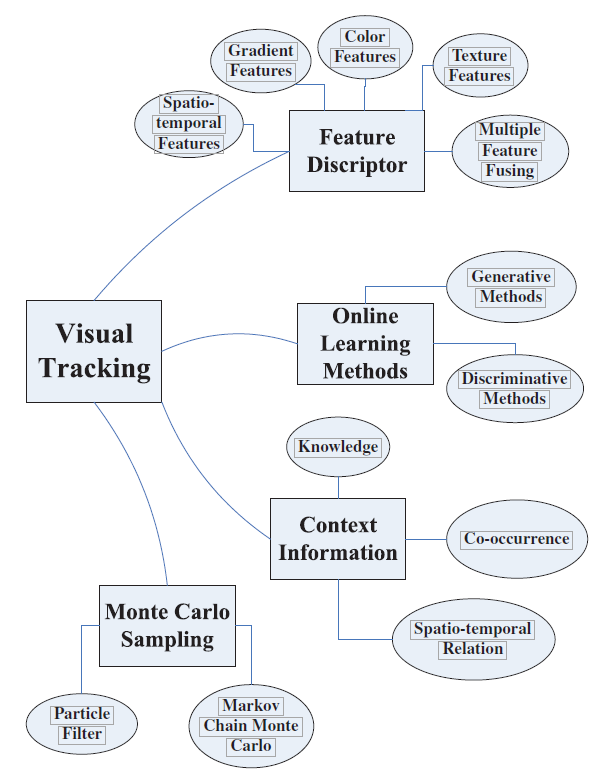
\includegraphics[width=0.45\linewidth]{figures/yang2011recent_graph.png}
   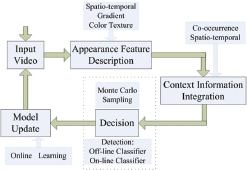
\includegraphics[width=0.45\linewidth]{figures/yang2011recent_flowchart.png}
   \caption{\textbf{Framework of tracking models}. From \cite{avidan2004support}.}
   \label{fig:yang2011recent}
\end{figure}


"State-of-the-art adaptive tracking-by-detection methods mainly
focus on improving tracking performance by increasing
the robustness of the classifier to poorly labelled samples
resulting from this approach. Examples of this include using
robust loss functions [6], [7], semi-supervised learning [8],
[9], or multiple-instance learning [3], [10]." \cite{hare2014struck}


% ====================
\section{Online RGB Trackers (vision papers)}
% ====================
Survey papers:
\begin{enumerate}
\item Yang et al. \cite{yang2011recent}. 2011 survey of the field
\item \textbf{Pang et al's Survey} \cite{pang2013finding} notes biases in
comparisons: usually new papers list their method as the best (because of a
specific methodology); however second best paper rankings are fairly robust. A
meta-analysis concludes the following methods are competitive: Struck, MIL, TLD,
VTD. 
\item \textbf{an extensive PAMI Survey} \cite{smeulders2013visual} claims Struck
is the best, and analyses specific failure cases and how it affects specific
method
\item \textbf{Appearance Model Survey} \cite{li2013survey}
\item A comprehensive list of papers can be found by searching papers that have
referenced Struck; which is the most frequently used benchmark to compare
against.
\item \textbf{Visual Tracking Benchmark}\cite{kristan2013visual} 
\item Wu et. al \cite{wu2013online} (SCM, Struck, TLD, ASLA, CXT, VTD, VTS, CSK)
concludes
    \begin{enumerate}
    \item \textbf{Background Information}  background
    information is critical for effective tracking. It can be ex-
    ploited by using advanced learning techniques to encode
    the background information in the discriminative model im-
    plicitly (e.g., Struck), or serving as the tracking contex-
    t explicitly (e.g., CXT)
    \item \textbf{local models}  are important for tracking as shown in the performance improvement of local sparse representation (e.g., ASLA and SCM) com-
    pared with the holistic sparse representation (e.g., MTT and
    L1APG). They are particularly useful when the appearance
    of target is partially changed, such as partial occlusion or
    deformation.
    \item \textbf{local models} motion model or dynamic model is cru-
    cial for object tracking, especially when the motion of target
    is large or abrupt. However, most of our evaluated tracker-
    s do not focus on this component. Good location predic-
    tion based on the dynamic model could reduce the search
    range and thus improve the tracking efficiency and robust-
    ness.
    \end{enumerate}
\item VOT2014 Results \cite{kristan2014visual}
\end{enumerate}

``The challenge considers single-camera, single-target, model-free, causal trackers, applied to short-term tracking. The model-free property means that the only supervised training example is provided by the bounding box in the first frame.  The short-term tracking means that the tracker does not perform re-detection after the target is lost. Drifting off the target is considered a failure. The causality means that the tracker does not use any future frames, or frames prior to re-initialization, to infer the object position in the current frame." \cite{kristan2014visual}

``In this paper, we focus on the problem of model-free online tracking of an object,
given only the object’s initial position and previous observations, within a tracking-bydetection
framework."\cite{zhang2014meem}

``Model drift occurs because factors like tracking failure, occlusions and misalignment
of training samples can lead to bad model updates. One remedy is to incorporate the first
frame template or prior knowledge in the online model update procedure [20,15]. However,
relying on a fixed model prior tends to restrict the tracker’s ability to handle large
object appearance changes. Other trackers [22,32,14] use a “censorship mechanism”
where an update is prevented when certain criteria are met (or not met). The detection
of good or bad updates usually relies upon smoothness assumptions for motion and
appearance changes, which are often violated in challenging scenarios. And once the
censorship mechanism fails, these trackers will either miss the chance to evolve or get
trapped in a background region, due to the fact that the model can only evolve forward,
without a mechanism to correct for past mistakes."\cite{zhang2014meem}

% --------------------
\subsection{Pre-CVPR 2013 Trackers}
% --------------------


\paragraph{Online RGB Trackers} require no prior knowledge of the object, and only a bounding box of the target on the original frame. 
A survey of tracking methods \cite{wu2013online} (SCM, Struck, TLD, ASLA, CXT, VTD, VTS, CSK), as well as papers following the survey \cite{supancic2013self}, show the following methods are competitive for this problem:
\begin{enumerate}
\item \textbf{Struck} \cite{hare2011struck}  uses a kernelized structured output SVM to directly learn displacement vectors. Gaussian kernel on 192 haar-like features. Struck's TPAMI paper \cite{hare2014struck}. 

Kernelization does most of the work, but structured SVM formulation avoids arbitrary hand-tuned parameters: "a large part of the performance gains... can be attributed to our use of a kernelised SVM rather than a boosting-based classifier."

``(previous) algorithms separate the adaptation phase of
the tracker into two distinct parts: (i) the generation and
labelling of samples; and (ii) the updating of the classifier."

``we make use of the structured output SVM
framework of Tsochantaridis et al. [15]. In particular, we
extend the online structured output SVM learning method
proposed by Bordes et al. [16], [17] and adapt it to the task
of adaptive object tracking."

\item \textbf{SCM} \cite{zhong2012robust} 
\item \textbf{TLD} \cite{kalal2012tracking} "We develop a novel learning method (P-N learning) which estimates the
errors by a pair of “experts”: (i) P-expert estimates missed detections, and (ii) N-expert estimates false alarms. The learning process is
modeled as a discrete dynamical system and the conditions under which the learning guarantees improvement are found. We describe
our real-time implementation of the TLD framework and the P-N learning.

\item \textbf{APG-L1} \cite{bao2012real} "l1 norm related minimization model".
\item \textbf{MIL} \cite{babenko2009visual} Older well-known tracker using multiple instance learning.
\item \textbf{CXT} \cite{dinh2011context} uses background context
\item \textbf{ASLA} \cite{jia2012visual} 
\item \textbf{Circulant} \cite{henriques2012exploiting} (TPAMI \cite{henriques2015tracking}) uses fourier transformed graham matrix to improve .

The fastest tracker in \cite{wu2013online}.

``a notable optimization
is to use a fast but inaccurate classifier to select promising
patches, and only apply the full, slower classifier on those
[18], [19]."

 


\item Zhang \cite{zhang2012real} "propose a projection to a fixed
random basis, to train a Naive Bayes classifier, inspired
by compressive sensing techniques."
\end{enumerate}


% --------------------
\subsection{Post-CVPR 2013 Trackers}
% --------------------
After Wu et. al's  survey \cite{wu2013online}, the following notable methods were also published:

\begin{enumerate}
\item \textbf{Self-paced learning} \cite{supancic2013self} "we show that an accurate appearance model is considerably more effective than a strong motion model". 
\item \textbf{MEEM} \cite{zhang2014meem} claims state-of-the-art over Struck, SCM, MIL.
\item \textbf{Xiang} \cite{xiang2014monocular}
\item \textbf{Occlusion and motion reasoning for long-term tracking} \cite{hua2014occlusion} "Struck fails in
the presence of long-term occlusions as well as severe viewpoint changes
of the object. In this paper we propose a principled way to combine occlusion and motion reasoning with a tracking-by-detection approach."
\item Color tracker \cite{danelljan2014adaptive} - the \textbf{best}.
\end{enumerate}

% --------------------
\subsection{Analysis}
% --------------------
Struck is a major paper, topping the benchmarks of Pang \cite{pang2013finding}, Wu \cite{wu2013online} and Smeulders \cite{smeulders2013visual}. Notably, newer papers aren't as well-tested and perhaps better. Struck is basically kernelized structured output SVMs, where $(x,y)$ are image patches and displacements. Most of the gains come from the kernelization, though.

Circulant trackers are really, quite good.



% =============================================
\section{Online RGB-D Trackers (vision papers)}
\label{sec:online}
% =============================================
\paragraph{Online RGB-D Trackers} no prior knowledge of the object.
Song et. al's survey \cite{song2013tracking}, show \textbf{incorporating depth into tracking beats the state of the art.} It shows \textbf{Struck} \cite{hare2011struck} and VTD are competitive.

\textbf{Gaussian Process Regression} \cite{gao2014transfer} beats struck and Song et. al's survey benchmarks.

% =============================================
\section{Trackers (robotics papers)}
\label{sec:trackers}
% =============================================
\begin{enumerate}
\item RSS 14: Anytime Tracking \cite{held2014combining}
\item RSS 14: DART Pose Estimation \cite{schmidt2014dart} (relevant?)
\item ICRA: Small Obstacle Discovery over Images \cite{kumar2014markov}: small object segmentation using RGB, since depth info doesn't give much.
\item ICRA 14: Tracking ping pong balls \cite{zhang2014spin} This paper proposes a way to observe and estimate ball's spin in real-time, and achieve an accurate prediction. Based on the fact that a spinning ball's motion can be separated into global movement and spinning respect to its center, we construct an integrated vision system to observe the two motions separately. With a pan-tilt vision system, the spinning motion is observed through recognizing the position of the brand on the ball and restoring the 3D pose of the ball. Then the spin state is estimated with the method of plane fitting on current and historical observations. With both position and spin information, accurate state estimation and trajectory prediction are realized via Extended Kalman Filter(EKF). 
\item ICRA 14: road scene segmentation \cite{huang2014road} "we first produce initial object hypotheses by clustering the sparse 3D point cloud. The image pixels registered to the clustered 3D points are taken as samples to learn each object's prior knowledge. The priors are represented by Gaussian Mixture Models (GMMs) of color and 3D location information only, requiring no high-level features. We further formulate the segmentation problem within a Conditional Random Field (CRF) framework, which incorporates the learned prior models, together with hard constraints placed on the registered pixels and pairwise spatial constraints to achieve final results. "
\item ICRA 14: Learning latent structure for activity recognition \cite{hu2014learning}. Good overview of basics.
\end{enumerate}
% =============================================
\section{Temporal Speech Data}
\label{sec:temporalspeech}
% =============================================
Structured prediction is used in temporal data such as speech recognition. This
has yet to fully permeate object tracking in videos.

RGB-D videos provide a unique set of data to images. Objects are more easily
segmented based on depth data (without transformation) alone. This can be seen
in LIDAR \cite{morton2013multi}.

It is often the case that 


% =============================================
\section{RGB-D Datasets}
% =============================================
\begin{enumerate}
\item Princeton RGB-D \cite{song2013tracking}
\item Wu et al. \cite{wu2013online}
\item Bigbird \cite{singh2014bigbird} (relevant?)
\end{enumerate}
% =============================================
\section{RGB-D Features}
% =============================================
\begin{enumerate}
\item Learning rich features from rgb-d images for object detection and segmentation \cite{gupta2014learning}
\item Segmentation using RGB-D data \cite{abramov2012depth}
\item Shotton's Random Forest \cite{shotton2013real}: ``each feature need only
read at most 3 image pixels and perform at most 5 arithmetic
operations; and the features can be straightforwardly implemented
on the GPU. Given a larger computational budget,
one could employ potentially more powerful features based
on, for example, depth integrals over regions, curvature, or
local descriptors"

\begin{figure}
   \hspace{-2mm}
   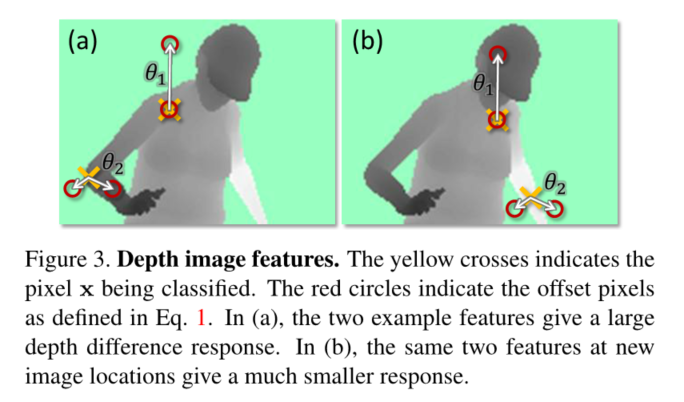
\includegraphics[width=0.45\linewidth]{figures/shotton2013real_features.png}
   \caption{\textbf{Shotton's Random Forest} \cite{shotton2013real}}
   \label{fig:shotton2013real_features}
\end{figure}
\end{enumerate}

% =============================================
\subsection{Shotton Random Forests}
% =============================================

% ====================
\section{Early Tracking}
% ====================
Tracking pre-2005ish.

CONDENSATION—Conditional Density Propagation for Visual Tracking: "The problem of tracking curves in dense visual clutter is challenging. Kalman filtering is inadequate because it is based on Gaussian densities which, being unimodal, cannot represent simultaneous alternative hypotheses. The CONDENSATION algorithm uses ``factored sampling'', previously applied to the interpretation of static images, in which the probability distribution of possible interpretations is represented by a randomly generated set. CONDENSATION uses learned dynamical models, together with visual observations, to propagate the random set over time. The result is highly robust tracking of agile motion. Notwithstanding the use of stochastic methods, the algorithm runs in near real-time."

http://www.cse.psu.edu/~rcollins/CollinsVLPR2012Lecture.pdf
http://www.cse.psu.edu/~rcollins/CollinsVLPR2009Lecture.pdf

% ====================
\section{Misc Other things}
% ====================

Pedestrian detection using optical flow. \cite{benenson2014ten}

\textbf{FABMAP}:
Bag of words,  descriptor, vector quantization into a visual word, Chow-liu trees for bayesian probability

% ====================
\section{Techniques}
% ====================
\begin{enumerate}
\item Structured SVMs: vedaldi2014structuredsvm
\item Multi-resolution \cite{park2010multiresolution}: for finite resolution cameras, scale variance is needed.
\end{enumerate}

% ====================
\section{Other Techniques}
% ====================
Gaussian Processes Bible (with matlab toolbox) \cite{rasmussen2006gaussian}
% --------------------

% --------------------
% ====================
\chapter{Method (My Idea)}
% ====================

% • In a paper you MUST provide the details, but FIRST convey the idea
% • Introduce the problem, and your idea, using EXAMPLES and only then
% present the general case
% • Explain it as if you were speaking to someone using a whiteboard
% • Conveying the intuition is primary, not secondary
% • Once your reader has the intuition, she can follow the details (but not vice
% versa)
% Even if she skips the details, she still takes away something valuable
% Evidence
% • Your introduction makes claims; The body of the paper provides evidence to
% support each claim
% • Check each claim in the introduction, identify the evidence, and forward-
% reference it from the claim
% • Evidence can be: analysis and comparison, theorems, measurements, case
% studies

% ====================
\section{My Idea (2 pages)}
% ====================

% ====================
\section{The details (5 pages)}
% ====================

% ====================
\chapter{Motion Planning}
% ====================
% --------------------
\section{Basic Ingredients}
% --------------------
\begin{itemize}
\item State
\item Time
\item Actions
\item Initial and Goal States
\item Feasibility and Optimality Criterion
\item A Plan
\end{itemize}

For a full description, see Chapter 1.3 of Lavalle \cite{lavalle2006planning}.
% --------------------
\section{Introduction to Motion Planning}
% --------------------
% --------------------
\subsection{Simple Motion Planning}
% --------------------
The simplest motion planning problems assume knowledge of a global map, a fixed
known goal state and a fixed known initial state. The problem is to determine a
feasible path from the initial state to the goal state. An optimality criterion
may also be applied to choose the best path if multiple feasible ones are found.

Notably, two important concepts have often been ignored in determining the path:
the dynamics of the system and the use of feedback. Dynamics refers to how
states transition to other states, and is inherent in real-world systems. For
example, a car can easily move fowards and backwards, but cannot immediately
move side to side. Feedback refers to the technique of refining further actions
based on newly sensed data. In simulations, feedback may not be necessary, but
in real-world systems, errors in sensing and modeling build up over time without
it.

In this simple case, the generated path is followed in an open-loop manner, or
if subject to real-world constraints (see \autoref{fig:lavalle2006planning119}),
the generated path is smoothed to obey the system's dynamics and feedback is
used to closely follow the path. "Notably this approach is highly decoupled as
feedback and dynamics are neglected in constructing the original path"
\cite{lavalle2006planning}. The smooth path may now obey the robot's dynamics,
but may no longer be feasible.  Feedback is used merely as an inefficient
afterthought.

\begin{figure}
\centering
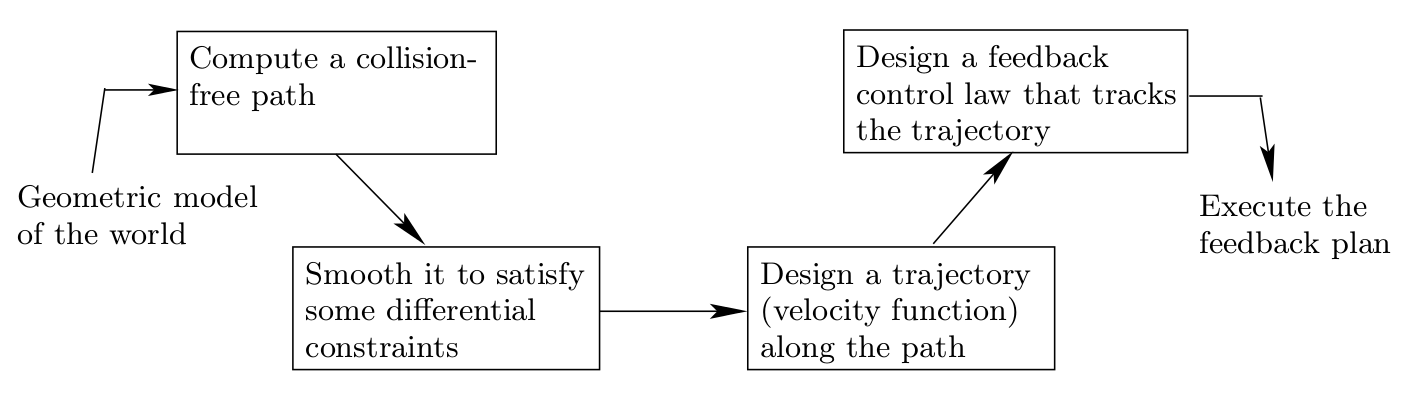
\includegraphics[width=3in]{figures/lavalle2006planning119.png}
\caption{From \cite{lavalle2006planning}. A refinement approach that has been used for decades in robotics.}
\label{fig:lavalle2006planning119}
\end{figure}

Even in this simple case, obtaining an optimal or even feasible path is not
straightforward if the state space is large. A* search for trivially sized state
spaces and sampling-based techniques such as RRTs (RRT* for optimality) and PRMs
have proven to be the methods of choice (citation?), though it is still an
ongoing field of interest (cite 2015 RRT/PRM papers).

% --------------------
\subsection{Feedback Motion Planning}
% --------------------
Dynamics refers, generally, to how a state transitions to another state.

Feedback (or reactive plans) refers to something else.

Tiers of motion planning problems
\begin{itemize}
\item Fixed Initial and Goal States, no dynamics, no feedback, some optimality
criterion: RRT*, PRM*
\item Fixed Initial and Goal States, dynamics, no feedback: RRT*, A*
\item Fixed Initial and Goal States, no dynamics, feedback
\end{itemize}

see \autoref{fig:determinedrive2}.
\begin{figure}
\centering
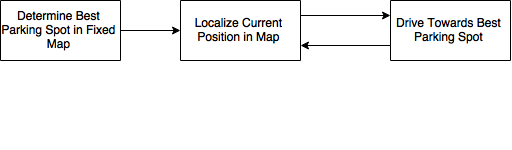
\includegraphics[width=3in]{figures/determinedrive2.png}
\caption{Feedback loop}
\label{fig:determinedrive2}
\end{figure}


% --------------------
\subsection{Feedback Motion Planning with Updating Goal State}
% --------------------
see \autoref{fig:determinedrive1}.
For a full description, see Chapter 8 of Lavalle \cite{lavalle2006planning}.

\begin{figure}
\centering
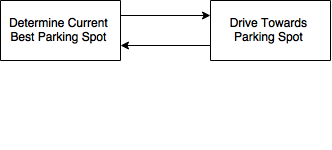
\includegraphics[width=3in]{figures/determinedrive1.png}
\caption{Feedback loop}
\label{fig:determinedrive1}
\end{figure}


% --------------------

% --------------------
\chapter{Experiments}
\label{ch:experiments}


% ====================
\section{Installing F}
% ====================

\begin{enumerate}
	\item implement princeton RGBD algorithm
	\item implement struck
	\item implement 2014 color tracking algorithm
	\item implemenmt Gaussian processes algorithm
\end{enumerate}

\subsubsection{Implementing the princeton "song2013tracking" RBGD algorith}

code is in song2013tracking. 

% --------------------



%\include{model}
%\include{impl}
%\include{discussion}
%\include{conclusions}

%    3. Notes
%    4. Footnotes

% --------------------
%    5. Bibliography
% --------------------
\begin{singlespace}
\raggedright
\bibliographystyle{abbrvnat}
\bibliography{biblio}
\end{singlespace}

% --------------------
\appendix
%    6. Appendices (including copies of all required UBC Research
%       Ethics Board's Certificates of Approval)
%\include{reb-coa}	% pdfpages is useful here
% --------------------
% ====================
\chapter{Metachapter: How to Do Research}
% ====================

% ====================
\section{How to do research}
% ====================
Todo: make into checklist form: How to do research \cite{chapman1988how}
\cite{hwang2008how}
\cite{desjardins2008how}

Chapman in 1988~\cite{chapman1988how}: informal rules of thumb advice. Each
section corresponds to a chapter in his document, in the same order.


% ====================
\section{How to read}
% ====================

Chapman~\cite{chapman1988how}:
\blockquote{Many researchers spend more than half their time reading}

\blockquote{The time to start reading is now. Once you start seriously working
on your thesis you’ll have less time, and your reading will have to be more
focused on the topic area. During your first two years, you’ll mostly be doing
class work and getting up to speed on AI in general. For this it suffices to
read textbooks and published journal articles.}

\blockquote{The reading lists for the AI qualifying exams at other
universities—particularly Stanford—are also useful}

\blockquote{There are three phases to reading. The
first is to see if there’s anything of interest in it at all. Second is to find
the part of the paper that has the good stuff. Most fifteen page papers could
profitably be rewritten as one-page papers; you need to look for the page that
has the exciting stuff. Often this is hidden somewhere unlikely. What the author
finds interesting about his work may not be interesting to you, and vice versa.
Finally, you may go back and read the whole paper through if it seems
worthwhile}

\blockquote{Read with a question in mind. “How can I use this?” “Does this really do
what the author claims?” “What if...?” Understanding what result has been presented
is not the same as understanding the paper. Most of the understanding
is in figuring out the motivations, the choices the authors made (many of them
implicit), whether the assumptions and formalizations are realistic, what directions
the work suggests, the problems lying just over the horizon, the patterns
of difficulty that keep coming up in the author’s research program, the political
points the paper may be aimed at, and so forth.}

\blockquote{If you are interested in an area and read a few papers about it, try
implementing toy versions of the programs being described. This gives you a more
concrete understanding.}

% --------------------
\subsection{Reading a paper checklist}
% --------------------

\begin{itemize}
\item How can I use this?
\item Does this really do what the author claims?
\item Are assumptions and formalizations realistic?
\item Implement a toy version of the program
\end{itemize}

% ====================
\section{Getting connected}
% ====================

Chapman~\cite{chapman1988how}:
\blockquote{it’s important to get plugged into the Secret Paper Passing Network.
This informal organization is where all the action in AI really is.}

This can be done by
\begin{itemize}
\item Mailing lists
\item Talk about an idea you’ve had with someone who knows the
field; they are likely to say, “Have you read X?” 
\item When you read a paper that excites you, send it to people who might be
interested in it. They'll return the favor.
\item Discussion groups
\item Read papers on people's desks, filing cabinets
\item Distribute draft copies of things you write (``Please do not photocopy or
quote" on the front page). Most people don’t read most of the papers they’re
given, so don’t take it personally
\item When you finish a paper, send copies to everyone you think might be
interested.
\item Make yourself the bridge between two groups of
interesting people working on related problems who aren’t talking to each
other
\item Keep a log of interesting references.
\item Try talking to them about the really good or unbelievably foolish stuff
you’ve been reading. Hang out, dinners, lunches, informal gatherings.
\item Get a business card.
\item At conferences, walk up to someone whose paper you’ve liked, say ``I really
liked your paper", and ask a question.
\item Get summer jobs away at other labs.
\end{itemize}

\blockquote{It’s important to get a variety of people who will regularly review
your work, because it's very easy to mislead yourself (and often your advisor as
well) into thinking you are making progress when you are not, and so zoom off
into outer space.}

% ====================
\section{Learning other fields}
% ====================
\begin{itemize}
\item Take a graduate course. This is solidest, but is often not efficient.
\item Read a textbook. Not a bad approach, but textbooks are usually out of date, and generally have a high ratio of words to content.
\item Find out what the best journal in the field is, maybe by talking to someone who knows about it. Then skim the last few years worth and follow the reference trees. This is usually the fastest way to get a feel of what is happening, but can give you a somewhat warped view.
\item Find out who’s most famous in the field and read their books.
\item Hang out with grad students in the field.
\item Go to talks. 
\end{itemize}

% ====================
\section{Keeping a Research Notebook}
% ====================
\blockquote{Record in your notebook ideas as they come up. Nobody except you is going
to read it, so you can be random. Put in speculations, current problems in your
work, possible solutions. Work through possible solutions there. Summarize for
future reference interesting things you read.}

Methods?
\begin{itemize}
\item HTML Website. Pros: easily accessed from the web. Cons: Hard to update
\item One big Latex file. Pros: easy to transfer to a paper. Cons: No
hyperlinks. I'll use this.
\end{itemize}

Vera Johnson-Steiner's book Notebooks of the Mind: Describes how creative
thought emerges from the accumulation of fragmented ideas.

% ====================
\section{Writing}
% ====================

% --------------------
\subsection{General}
% --------------------
\blockquote{Writing down your ideas is the best way to debug them. Usually you will
find that what seemed perfectly clear in your head is in fact an incoherent
mess on paper.

Realize that writing is
a debugging process. Write something sloppy first and go back and fix it up.
Starting sloppy gets the ideas out and gets you into the flow. If you “can’t”
write text, write an outline. Make it more and more detailed until it’s easy
to write the subsubsubsections. If you find it really hard to be sloppy, try
turning the contrast knob on your terminal all the way down so you can’t
see what you are writing. Type whatever comes into your head, even if it
seems like garbage. After you’ve got a lot of text out, turn the knob back
up and edit what you’ve written into something sensible.

Perfectionism can also lead to endless repolishing of a perfectly adequate
paper. This is a waste of time. (It can also be a way of semideliberately
avoiding doing research.) 
}

List of papers that are well-written:
\begin{itemize}
\item None so far!
\end{itemize}

List of poorly written papers/quotes:
\begin{itemize}
\item None so far!
\end{itemize}

General tips:
\begin{itemize}
\item Put the sexy stuff up front, at all levels of organization from paragraph
up to the whole paper.
\item explain why it works and why it’s interesting
\item Do not imitate math texts; their standard of elegance is to say as little
as possible, and so to make the reader’s job as hard as possible. This is not
appropriate for AI.
\item After you have written a paper, delete the first paragraph or the first few
sentences. You’ll probably find that they were content-free generalities, and
that a much better introductory sentence can be found at the end of the
first paragraph of the beginning of the second.
\end{itemize}

% --------------------
\subsection{Goals for Getting Published}
% --------------------
Standards are surprisngly low.
Criteria:
\begin{itemize}
\item Has something new to say
\item Isn't broken in some way
\end{itemize}

Strategies:
\begin{itemize}
\item Try a lot
\item Make sure it's readable
\item Circulate drafts beforehand
\item Read backissues of conference and make sure style/content is appropriate
\item Read the information for authors page specified by conference
\item Read best paper awards
\end{itemize}

% --------------------
\subsection{Abstract}
% --------------------
Print this off and use this as a checklist whenever I write a paper.
Stuff from Simon Peyton-Jones' talk~\cite{jones2013how}.

\begin{itemize}
\item Four sentences:
\item state the problem
\item state why it's an interesting problem
\item say what your solution achieves
\item say what follows from your solution
\end{itemize}

% --------------------
\subsection{Intro}
% --------------------
\begin{itemize}
\item (1 page in conference)
\item Describe the problem
\item State your contributions (write the list of contributions fist)
\item that's all
\item use an example to introduce the problem
\item Reader thinks``gosh, if they can really deliver this, that'd be exciting; I’d better read on" \cite{jones2013how}
\item Contributions should be refutable
\item No "the rest of the paper is". Instead, use forward references from the narrative in the introduction. The introduction (including the contributions) should survey the whole paper, and therefore forward reference every important part
\end{itemize}

% --------------------
\subsection{The Problem}
% --------------------
\begin{itemize}
\item 1 page
\end{itemize}

% --------------------
\subsection{Related Work Purpose (1-2 pages)}
% --------------------
\begin{itemize}
\item show my problem is unsolved
\item show my problem is interesting
\item show my idea works
\item show how my idea compares to other ideas
\end{itemize}

\begin{itemize}
\item No related work yet! Include at end.
\begin{itemize}
    \item Problem 1: describing alternative approaches gets between the reader and your idea (I feel tired)
    \item Problem 2: the reader knows nothing
    about the problem yet; so your (carefully
    trimmed) description of various technical
    tradeoffs is absolutely incomprehensible (I feel stupid)
    \item instead, Concentrate single-mindedly on a narrative that
    \begin{itemize}
        \item Describes the problem, and why it is interesting
        \item Describes your idea
        \item Defends your idea, showing how it solves the problem,
and filling out the details
        \item On the way, cite relevant work in passing, but defer
discussion to the end
    \end{itemize}
\end{itemize}

\item show how my idea compares to other ideas
\item Be generous to the competition. “In his inspiring paper
[Foo98] Foogle shows.... We develop his foundation in the
following ways...
\item Giving credit to others does not diminish
the credit you get from your paper
\item Acknowledge weaknesses in your approach
\item Failing to give credit to others can kill
your paper: You don't know that it's an old idea (bad) or You do know, but are pretending it's yours (very bad)

\item 

\end{itemize}

% --------------------
\subsection{Method}
% --------------------
\begin{itemize}
\item In a paper you MUST provide the details,
but FIRST convey the idea
\item Introduce the problem, and your idea, using
EXAMPLES and only then present the general case
\item Explain it as if you were speaking to someone using
a whiteboard
\item Conveying the intuition is primary, not secondary
\item Once your reader has the intuition, she can follow
the details (but not vice versa)
\item Even if she skips the details, she still takes away
something valuable
\end{itemize}

Evidence
\begin{itemize}
\item Your introduction makes claims; The body of the paper provides evidence to support each claim
\item Check each claim in the introduction, identify the
evidence, and forward-reference it from the claim
\item Evidence can be: analysis and comparison, theorems,
measurements, case studies
\end{itemize}


% ====================
\section{Giving Talks}
% ====================
\blockquote{Since revising a talk is generally much easier than revising a
paper, some people find that this is a good way to find the right way to express
their ideas. (Mike Brady once remarked that all of his best papers started out
as talks.)}

\blockquote{Cornering one of your friends and trying to explain your most recent
brainstorm to him is a good way both to improve your communication skills, and
to debug your ideas.}




% ====================
\section{Programming}
% ==================== 
\blockquote{Like papers, programs can be over-polished. Rewriting code till it’s
perfect, making everything maximally abstract, writing macros and libraries, and
playing with operating system internals has sucked many people out their theses
and out of the field.}

% ====================
\section{How to Select a Graduate Advisor}
% ====================
\begin{itemize}
\item How much direction do you want? 
\item How much contact do you want? 
\item How much pressure do you want? 
\item How much emotional support do you want? 
\item How seriously do you want to take your advisor? 
\item What kind of research group does the advisor provide? 
\item Do you want to be working on a part of a larger project? 
\item Do you want cosupervision? 
\item Is the advisor willing to supervise a thesis on a topic outside his main area of research? 
\item Will the advisor fight the system for you? 
\item Is the advisor willing and able to promote your work at conferences and the like? 
\end{itemize}


\begin{itemize}
\item Read the Lab’s research summary. 
\item Read recent papers of any faculty member whose work seems at all interesting.
\item Talk to as many faculty members as you can during your first semester.
\item Talk to grad students of prospective advisors and ask what working for him or her is like. 
\item Attend faculty member's research group meetings
\end{itemize}

% ====================
\section{How to Choose a Thesis Topic and Avoid Wasting Time}
% ====================
\blockquote{The essential requirement of a Master’s thesis is that it literally
demonstrate mastery: that you have fully understood the state of the art in your
subfield and that you are capable of operating at that level. It is not a
requirement that you extend the state of the art, nor that the Master’s thesis
be publishable.

The actual writing of the PhD thesis generally takes about a year, and an
oft-confirmed rule of thumb is that it will drag on for a year after you are
utterly sick of it.
}

Read other people's theses.

Choosing a topic:
\begin{itemize}
\item A good thesis topic will simultaneously express a personal vision and participate in a conversation with the literature.
\item Your topic must be one you are passionate about. Nothing less will keep you going. Your personal vision is your reason for being a scientist, an image or principle or idea or goal you care deeply about. It can take many forms. Maybe you want to build a computer you can talk to. Maybe you want to save the world from stupid uses of computers. Maybe you want to demonstrate the unity of all things. Maybe you want to found colonies in space. A vision is always something big. Your thesis can’t achieve your vision, but it can point the way.
\item At the same time, science is a conversation. An awful lot of good people have done their best and they’re written about it. They’ve accomplished a great deal and they’ve completely screwed up. They’ve had deep insights and they’ve been unbelievably blind. They’ve been heros and cowards. And all of this at the same time. Your work will be manageable and comprehensible if it is framed as a conversation with these others. It has to speak to their problems and their questions, even if it’s to explain what’s wrong with them.  A thesis topic that doesn’t participate in a conversation with the literature will be too big or too vague, or nobody will be able to understand it.
\item The hardest part is figuring out how to cut your problem down to a solvable size while keeping it big enough to be interesting. “Solving AI breadth-first” is a common disease; you’ll find you need to continually narrow your topic.  Choosing a topic is a gradual process, not a discrete event, and will continue up to the moment you declare the thesis finished. Actually solving the problem is often easy in comparison to figuring out what exactly it is. If your vision is a fifty-year project, what’s the logical ten-year subproject, and what’s the logical one-year subproject of that? If your vision is a vast structure, what’s the component that gets most tellingly to its heart, and what demonstration would get most tellingly to the heart of that component?
\item An ideal thesis topic has a sort of telescoping organization. It has a central portion you are pretty sure you can finish and that you and your advisor agree will meet the degree requirements. It should have various extensions that are successively riskier and that will make the thesis more exciting if they pan out. Not every topic will fit this criterion, but it’s worth trying for.
\item Some people find that working on several potential thesis projects at once allows them to finish the one that works out and abandon the ones that fail.
\item Topics can be placed in a spectrum from flakey to cut-and-dried. Flakier theses open up new territory, explore previously unresearched phenomena, or suggest heuristic solutions to problems that are known to be very hard or are hard to characterize. Cut-and-dried theses rigorously solve wellcharacterized problems. Both are valuable; where you situate yourself in this spectrum is a matter of personal style.
\item The “further work” sections of papers are good sources of thesis topics.
\end{itemize}


be able to explain simply how each part of your theory
and implementation is in service of the goal.

Make sure once you’ve selected a topic that you get a clear understanding with
your advisor as to what will constitute completion.

Try a simplified version of the thesis problem first. Work examples. Thoroughly
explore some concrete instances before making an abstract theory

There are a number ways you can waste a lot of time during the thesis. Some
activities to avoid (unless they are central to the thesis): language design, userinterface
or graphics hacking, inventing new formalisms, overoptimizing code, tool
building, bureaucracy. Any work that is not central to your thesis should be
minimized.
% ====================
\section{How to do Resarch Methodology}
% ====================

% ====================
\section{Emotional Factors in the Research Process}
% ====================

The entire section by Chapman~\cite{chapman1988how} is worth a read.

Biograpahies: Gregory Bateson’s Advice to a Young Scientist, Freeman Dyson’s
Disturbing the Universe, Richard Feynmann’s Surely You Are Joking, Mr.
Feynmann!, George Hardy’s A Mathematician’s Apology, and Jim Watson’s The Double
Helix

\chapter{Daily Log}

% --------------------
\section{2014 December}
% --------------------

To do:
\begin{itemize}
\item RPE intial draft
\item Giraffe paper camera-ready copy
\end{itemize}

Done:
\begin{itemize}
\item none!
\end{itemize}



\chapter{Supporting Materials}

This would be any supporting material not central to the dissertation.
For example:
\begin{itemize}
\item additional details of methodology and/or data;
\item diagrams of specialized equipment developed.;
\item copies of questionnaires and survey instruments.
\end{itemize}

\chapter{Career}
\label{ch:career}

% ====================
\section{Questions for Job Fairs}
% ====================
As a busy student, how do you keep up to date with technology developments in industry? 
What was the last technology that you heard of and thought 'that's really cool'? 'uncool'? 
Suppose you're locked in a building and can't leave. How many ways can you think of to measure the exterior temperature? 
Resume related questions: Fairtunes, C\&O, Waterloo. 
How can you prevent deadlock in a concurrent system? 
Write a function to add 64 bit numbers using 32bit arithmetic. 
What is a thread? What is a process? 
Write a function that, given an alphabetic string, outputs the characters a) sorted b) duplicates removed and c) in lower case. Do it using only a few (<26) bytes of storage. (eg: "Mississippi" -> "imps") 
Insert into a circular doubly linked list. 
A square island, with side length n meters, lies in the center of a square pond, with side length n+2 meters. Given only two boards of length 0.99 meters, how can you reach the island from the mainland? 
ASCII strings are typically encoded using 1 byte per character, even though for alphanumeric text, only the first 7 bits are used (the MSB is always 0). Write a function that compresses a c string by outputting a string of bytes where each group of seven bits represents each character of input. For example, the 3 byte string 01111111, 01011100, 00000101 would compress to the 21 bit string 111111110111000000101. 
itoa() (He first suggested "reverse the word ordering in a string", then malloc()/free()) 
Tell me about a time your beliefs were challenged in the workplace. 
Tell me about a time when you discovered a fundamental error in the design of your project. 
Design and implement the "shuffle" function for a 200 disc CD changer. Your only constraint is that no song may be repeated until every other song has been played once. 

% ====================
\section{Questions for Interviews}
% ====================

% ====================
\section{Job Fair}
% ====================

Look professional, smile, clear and confident-sounding voice, a firm handshake
and good eye contact. Wear my blue shirt, perhaps get it tailored.

\paragraph{Introduction} Hi, I'm Victor. I'm a second year Master's student in Computer Science doing
research in Robotics and Computer Vision. I'll be looking for full-time
positions starting in September. Does [company] have any opportunities in
software development?

Questions to learn about company culture, organization:
\begin{itemize}
    \item What's pretty hot to know nowadays in Microsoft? What programming
    languages?
    \item Are there code reviews?
    \item On your 'About us' section of your webpage you mention X.
    \item I printed out a copy of a job description on your website. What do you
    mean by 'you need X?'
    \item How do you like your team? Can new hires meet potential teams?
\end{itemize}

\paragraph{Follow up email} Hi John, it was greating speaking with you at the
UBC Technical Career Fair last Wednesday. Thanks for telling me about the
machine learning positions at Microsoft. As mentioned, I'll be looking for
full-time positions starting in September and the positions you've describe seem
like a good fit for me. Here's a copy of the resume I gave you. Feel free to
reach me at 2369997236 or this email address, vhg@cs.ubc.ca.


% ====================
\section{Misc Resources}
% ====================

\url{https://www.cs.ubc.ca/students/undergrad/careers/finding/preparing-technical-career-fair-tips}

\url{http://www.reddit.com/r/cscareerquestions/comments/20ahfq/heres_a_pretty_big_list_of_programming_interview/}:
\blockquote{You probably could get away with a single page cheatsheet but beyond that you probably will be spending more time looking things up and that will count against you. The questions are also very academic in nature but still application oriented so you need to know when, where, and how to use all the different data structures and quickly adapt them to your needs in the question. They will then ask you about performance and a bunch of other things(at least in my interviews) so in order to have a complete cheat sheet you need to have or remember everything you probably learned in your first 2 years of CS classes feeding on your last 2 years of classes. The recruiter I talked to said people at Google said that the phone interview and the process in general was harder than the hardest test they had in school but very similar to a final exam for one of their classes.
}


• Be well prepared, study hard.
• Buy a few good books
• Cracking the Coding Interview
• Programming Interviews Exposed
• How Would You Move Mount Fuji?
• Talk to friends.
• Aggressively pursue interview opportunities. They rarely come to you.
• Make sure you can perform well with little to no sleep.
• Know what they want. Then show you have that.
• Enjoy the game.
• Contact HR if you haven’t heard from them (see JC Oct 6).
• Be enthusiastic.
• No two interview experiences are alike. Prepare for anything and everything.
• Research shows that the interviewer makes up their mind in the first thirty seconds that they meet you.
• Don’t have a cover letter.
• Be honest with yourself and your interviewers.



% ====================
\section{Interview Questions}
% ====================
\subsection{How to Answer Interview Questions}
\blockquote{As an interviewer, I would expect you to know proper syntax for
common things in whatever language you work in (presumably Java), as well as
very common API (substring, working with collections, etc). If you can't write a
for loop, then that would be problematic. Don't know the try-with-resources
syntax? That's OK. If you don't know that substring exists, problem. If you use
"put" instead of "add" (or vice versa) for a collection - not a big deal, that's
what IDEs are for. And even if you mess up on something basic, if you still did
fine on the rest of it, I'll overlook that.}

Algorithm:
\begin{enumerate}
\item Ask clarifying questions
\item Give an example and verify: simple example
\item Give an example and verify: corner case
\item Think about possible solutions and complexity
\item Lower bound complexity
\item Start writing
\item Walk through code
\item Test with: Simple example (walk through code exactly)
\item Test with: b. Corner cases
\end{enumerate}

\subsection{General}
\begin{itemize}
\item Find the most frequent integer in an array
\item Find pairs in an integer array whose sum is equal to 10 (bonus: do it in linear time)
\item Given 2 integer arrays, determine of the 2nd array is a rotated version of the 1st array. Ex. Original Array A={1,2,3,5,6,7,8} Rotated Array B={5,6,7,8,1,2,3}
\item Write fibbonaci iteratively and recursively (bonus: use dynamic programming)
\item Find the only element in an array that only occurs once.
\item Find the common elements of 2 int arrays
\item Implement binary search of a sorted array of integers
\item Implement binary search in a rotated array (ex. {5,6,7,8,1,2,3})
\item Use dynamic programming to find the first X prime numbers
\item Write a function that prints out the binary form of an int
\item Implement parseInt
\item Implement squareroot function
\item Implement an exponent function (bonus: now try in log(n) time)
\item Write a multiply function that multiples 2 integers without using *
\item HARD: Given a function rand5() that returns a random int between 0 and 5, implement rand7()
\item HARD: Given a 2D array of 1s and 0s, count the number of "islands of 1s" (e.g. groups of connecting 1s)
\end{itemize}
\subsection{Strings}
\begin{itemize}
\item Find the first non-repeated character in a String
\item Reverse a String iteratively and recursively
\item Determine if 2 Strings are anagrams
\item Check if String is a palindrome
\item Check if a String is composed of all unique characters
\item Determine if a String is an int or a double
\item HARD: Find the shortest palindrome in a String
\item HARD: Print all permutations of a String
\item HARD: Given a single-line text String and a maximum width value, write the function 'String justify(String text, int maxWidth)' that formats the input text using full-justification, i.e., extra spaces on each line are equally distributed between the words; the first word on each line is flushed left and the last word on each line is flushed right
\end{itemize}
\subsection{Trees}
\begin{itemize}
\item Implement a BST with insert and delete functions
\item Print a tree using BFS and DFS
\item Write a function that determines if a tree is a BST
\item Find the smallest element in a BST
\item Find the 2nd largest number in a BST
\item Given a binary tree which is a sum tree (child nodes add to parent), write an algorithm to determine whether the tree is a valid sum tree
\item Find the distance between 2 nodes in a BST and a normal binary tree
\item Print the coordinates of every node in a binary tree, where root is 0,0
\item Print a tree by levels
\item Given a binary tree which is a sum tree, write an algorithm to determine whether the tree is a valid sum tree
\item Given a tree, verify that it contains a subtree.
\item HARD: Find the max distance between 2 nodes in a BST.
\item HARD: Construct a BST given the pre-order and in-order traversal Strings
\end{itemize}
\subsection{Stacks, Queues, and Heaps}
\begin{itemize}
\item Implement a stack with push and pop functions
\item Implement a queue with queue and dequeue functions
\item Find the minimum element in a stack in O(1) time
\item Write a function that sorts a stack (bonus: sort the stack in place without extra memory)
\item Implement a binary min heap. Turn it into a binary max heap
\item HARD: Implement a queue using 2 stacks
\end{itemize}
\subsection{Linked Lists}
\begin{itemize}
\item Implement a linked list (with insert and delete functions)
\item Find the Nth element in a linked list
\item Remove the Nth element of a linked list
\item Check if a linked list has cycles
\item Given a circular linked list, find the node at the beginning of the loop. Example: A-->B-->C --> D-->E -->C, C is the node that begins the loop
\item Check whether a link list is a palindrome
\item Reverse a linked list iteratively and recursively
\end{itemize}
\subsection{Sorting}
\begin{itemize}
\item Implement bubble sort
\item Implement selection sort
\item Implement insertion sort
\item Implement merge sort
\item Implement quick sort
\end{itemize}

\subsection{Dynamic Programming}
From \url{http://en.wikipedia.org/wiki/Dynamic_programming#Algorithms_that_use_dynamic_programming}:
\begin{itemize}
\item Recurrent solutions to lattice models for protein-DNA binding
\item Backward induction as a solution method for finite-horizon discrete-time dynamic optimization problems
\item Method of undetermined coefficients can be used to solve the Bellman equation in infinite-horizon, discrete-time, discounted, time-invariant dynamic optimization problems
\item Many string algorithms including longest common subsequence, longest increasing subsequence, longest common substring, Levenshtein distance (edit distance)
\item Many algorithmic problems on graphs can be solved efficiently for graphs of bounded treewidth or bounded clique-width by using dynamic programming on a tree decomposition of the graph.
\item The Cocke–Younger–Kasami (CYK) algorithm which determines whether and how a given string can be generated by a given context-free grammar
\item Knuth's word wrapping algorithm that minimizes raggedness when word wrapping text
\item The use of transposition tables and refutation tables in computer chess
\item The Viterbi algorithm (used for hidden Markov models)
\item The Earley algorithm (a type of chart parser)
\item The Needleman–Wunsch and other algorithms used in bioinformatics, including sequence alignment, structural alignment, RNA structure prediction
\item Floyd's all-pairs shortest path algorithm
\item Optimizing the order for chain matrix multiplication
\item Pseudo-polynomial time algorithms for the subset sum and knapsack and partition problems
\item The dynamic time warping algorithm for computing the global distance between two time series
\item The Selinger (a.k.a. System R) algorithm for relational database query optimization
\item De Boor algorithm for evaluating B-spline curves
\item Duckworth–Lewis method for resolving the problem when games of cricket are interrupted
\item The value iteration method for solving Markov decision processes
\item Some graphic image edge following selection methods such as the "magnet" selection tool in Photoshop
\item Some methods for solving interval scheduling problems
\item Some methods for solving word wrap problems
\item Some methods for solving the travelling salesman problem, either exactly (in exponential time) or approximately (e.g. via the bitonic tour)
\item Recursive least squares method
\item Beat tracking in music information retrieval
\item Adaptive-critic training strategy for artificial neural networks
\item Stereo algorithms for solving the correspondence problem used in stereo vision
\item Seam carving (content aware image resizing)
\item The Bellman–Ford algorithm for finding the shortest distance in a graph
\item Some approximate solution methods for the linear search problem
\item Kadane's algorithm for the maximum subarray problem
\end{itemize}


% --------------------
\backmatter
%    7. Index
% See the makeindex package: the following page provides a quick overview
% <http://www.image.ufl.edu/help/latex/latex_indexes.shtml>
% --------------------


\end{document}
